\documentclass[xcolor=pdftex,x11names,table,hyperref]{beamer}

\usepackage{verbatim}
\usepackage{setspace}
\usepackage{graphbox}
\usepackage{url}
\usepackage{xcolor} % See documentation PDF at http://www.ctan.org/pkg/xcolor
\definecolor{darkgreen}{rgb}{0,0.3,0}
\definecolor{darkblue}{rgb}{.05,.05,.30}
\definecolor{lightgrey}{rgb}{0.65,0.65,0.65}
\usepackage{tikzsymbols}


\setbeamertemplate{section in toc}[sections numbered]
\setbeamertemplate{subsection in toc}[subsections numbered]
\setbeamertemplate{subsubsection in toc}[subsubsections numbered]
\usetheme{Singapore}
\setbeamertemplate{navigation symbols}{}
\setbeamertemplate{footline}{%
\vspace{0.0em}%
\hspace{0.5em}%
{\color[rgb]{.1,.1,.1} \insertframenumber{}~/~\inserttotalframenumber}
}

\newcommand{\code}[1]{{\color{darkgreen}\texttt{#1}}}
\newcommand{\detail}[1]{{\color{lightgrey}\small{}#1}}
\newcommand{\teeny}[1]{\scalebox{0.17}{#1}}
\newcommand{\tablecolors}{\rowcolors{2}{blue!12}{white}} % Cool table colors

\newcommand{\actfun}[1]{\includegraphics[height=0.11\textheight,align=c]{images/#1}} % For consistency

\begin{document}

\title{Neural Networks \\[1.5em]
 %
\includegraphics[width=0.5\textwidth]{images/kitten_string_flickr_albaraa.jpg} \\[-1.0em]
 \small{Part 2} \\[1.0em]
 %LT1 \\[1.0em]
 }
\author{\href{http://jon.dehdari.org}{Jon Dehdari}}
\frame{\titlepage}

\begin{frame}{Good Morning!}
	\begin{center}
	%\includegraphics[width=0.8\textwidth]{images/.jpg}
	\end{center}
\end{frame}


% automatic differentiation of graph, why it's nice
%\begin{frame}{}
%\begin{itemize}
%	\item 
%	\item 
%\end{itemize}
%\end{frame}

% discussion of softmax, class-based decomp, hier softmax
\begin{frame}\frametitle{Softmax Normalization}

% http://tex.stackexchange.com/a/54007
\begin{minipage}[0.8\textheight]{\textwidth}
\begin{columns}[T]
\begin{column}{0.6\textwidth}
\begin{itemize}
	\item The slowest part of training a neural net LM is softmax normalization
	\item Why?  Before the softmax layer (final layer) we just have a real number, not a probability
	\item So we need to know the sum of scores for all possible words being predicted (ie. the normalization constant)
\end{itemize}
\end{column}
\begin{column}{0.6\textwidth}
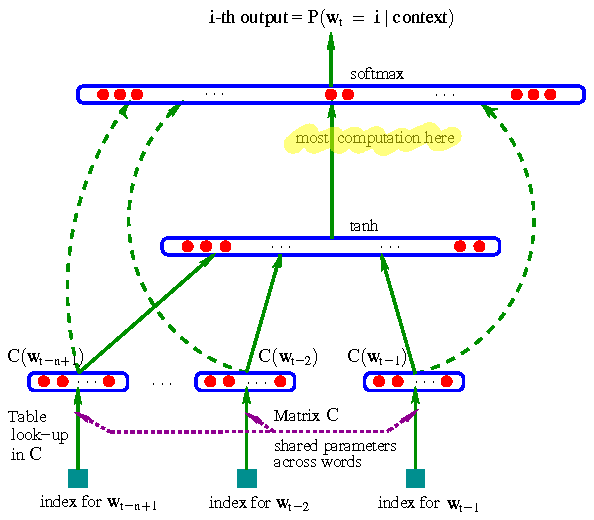
\includegraphics[width=1.0\textwidth]{images/bengio-etal2003_pg6_image_alt2.pdf}
\end{column}
\end{columns}
\end{minipage}

\pause

\hspace*{-2.0em}%
\begin{minipage}{1.0\textwidth}
\begin{itemize}
	\item This involves $|V|$ steps, where $|V|$ is the size of the vocabulary
	\item Typical values of $|V|$ are between 10K to 10M
	\item We must do this for every word in our training set (eg.\ 1M--1B), every epoch ($>10$)
\end{itemize}
\end{minipage}

\end{frame}


\begin{frame}{Speeding Up Normalization}
\begin{itemize}[<+->]
	\item Can we speed up normalization? We can approximate it:
	\item \textbf{Class-based Decomposition} works like class-based LMs: first determine prob.\ of a given word's class/POS, then the prob.\ of the specific word \detail{$\mathcal{O} ( \sqrt{|V|} )$}
	\item \textbf{Hierarchical Softmax} extends this idea to a fully binary-branching hierarchy of the vocabulary (like an ontology) \detail{$\mathcal{O} (\log_2(|V|) ) $ }
	\item \textbf{Noise Contrastive Estimation} (NCE) disposes with MLE (in Softmax).  Instead, a binary classifier is learned: observed training data vs.\ artificially generated noise.  word2vec's negative sampling is a simplified version. \detail{$\mathcal{O} (1) $}
	\item \textbf{Self Normalization} ensures that the normalization constant $Z$ is close to one. Slow for training, fast for test-time queries
\end{itemize}
\end{frame}

% Second set: recurrent NN's (Elman (vanishing/exploding gradient), GRU, LSTM), BPTT, maybe convolutional nets
% http://deeplearning.net/tutorial/lstm.html
% http://arxiv.org/pdf/1412.3555v1.pdf
% https://colah.github.io/posts/2015-08-Understanding-LSTMs/
% https://www.tensorflow.org/versions/master/tutorials/recurrent/index.html#recurrent-neural-networks
% https://www.ling.ohio-state.edu/~jonsafari/teaching/uds/lm/pres_09_rnnlm.pdf
% http://keras.io/layers/recurrent/
% https://en.wikipedia.org/wiki/LSTM

\begin{frame}{Recurrent Neural Networks for Sequential Data}
\begin{itemize}
	\item Feedforward (FF) networks only indirectly deal with sequential data (like language)
	\item FF Neural LMs are basically `soft' $n$-gram LMs -- their history is still fixed
	%\pause
	\item The model needs to `remember' a longer history, with loops:
\end{itemize}
\begin{center}
\begin{tiny}
%\begin{scalebox}{0.6}{
%\usepackage[hyperref,table,x11names]{xcolor} % See documentation PDF at http://www.ctan.org/pkg/xcolor
\usetikzlibrary{matrix,arrows,positioning,automata,shadows,shapes.geometric,shapes.misc}
\definecolor{darkblue}{rgb}{.05,.05,.30}
\definecolor{darkgreen}{rgb}{.05,.30,.05}
\definecolor{darkred}{rgb}{.30,.05,.05}

\hspace*{-3em}%
 \begin{tikzpicture}[->, >=stealth, line cap=round, shorten >=.4em, auto, node distance=8.0em, semithick, initial text={},]
   \tikzstyle{every state}=[rounded corners=.3em, rectangle, fill=darkblue, draw=none, text=white, drop shadow, minimum width=11em, hidden/.style ={white!95!black,text=black,minimum width=8em},]
   \tikzstyle{every path}=[line width=.15em]

   \node[state] (output_orig) {Output};
   \node[state,hidden] (hidden_orig) [below of=output_orig] {State/Hidden};
   \node[state] (input_orig) [below left=8em of hidden_orig.south east] {Input};
   \node[state,hidden] (previous) [below right=8em of hidden_orig.south west] {Previous State};


   \path


  (hidden_orig)
    edge [] node {$W$} (output_orig)
  (input_orig)
    edge [] node {$V$} (hidden_orig)
  (previous)
    edge [] node {$U$} (hidden_orig)
  (hidden_orig)
    edge [bend left=90] node {Copy (delayed)} (previous)
   ;
 \end{tikzpicture}

%}
\end{tiny}
\end{center}
\end{frame}





% \begin{frame}{}
% \begin{itemize}
% 	\item 
% 	\item 
% 	\item 
% \end{itemize}
% \end{frame}


\end{document}
